\lesson{Equilibrium Introduction}
\begin{bulleted-list}
    \item \textbf{Dynamic equilibrium:} a balance between forward and reverse processes occuring
        at the same rate. Requirements for dynamic equilibrium:
        \begin{enum}
            \item The system is a closed system
            \item All components of the chemical system need to be present
            \item The initial concentration of the chemicals stays the same throughout
        \end{enum}
    \item \textbf{Solubility equilibrium:} a dynamic equilibrium between a solute and a solvent
        in a saturated solution in a closed system
    \item \textbf{Phase equilibrium:} a dynamic equilibrium between different physical states of a
        pure substance in a closed system
    \item \textbf{Chemical reaction equilibrium:} a dynamic equilibrium between reactants and products
        of a chemical reaction in a closed system
\end{bulleted-list}

\begin{figure}[ht!]
    \centering
    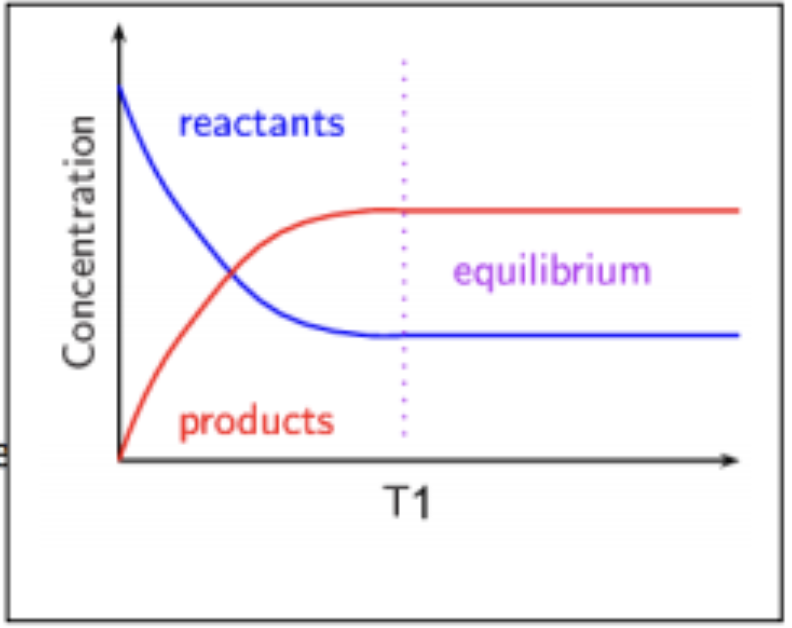
\includegraphics[width=0.3 \textwidth]{../figures/chemical-reaction-equilibrium-1.png}
    \caption{The position of the equilibrium shows that the products are more favoured. This means
    the percent reaction for reactants is less than 50\% and the percent reaction for
    products is greater than 50\%.}
    \label{fig:chemical-reaction-equilibrium-1}
\end{figure}

\begin{figure}[ht!]
    \centering
    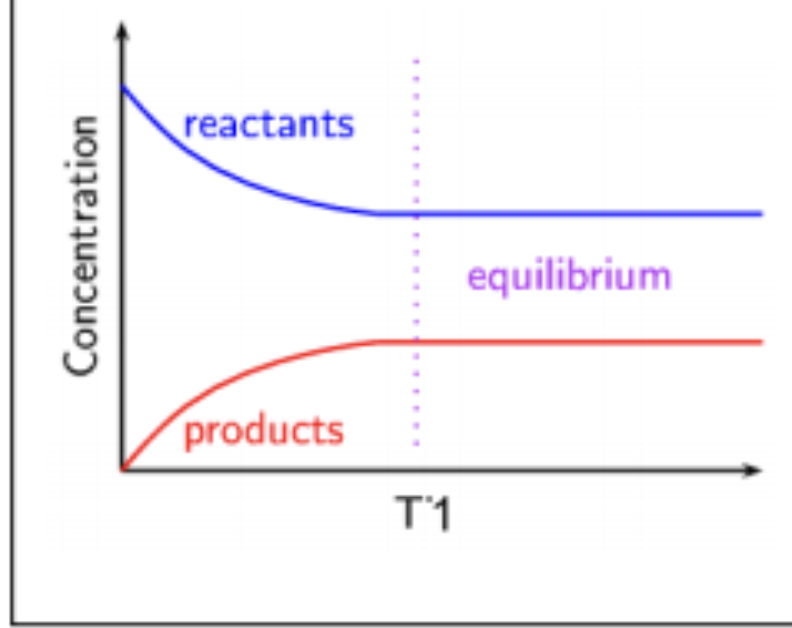
\includegraphics[width=0.3 \textwidth]{../figures/chemical-reaction-equilibrium-2.png}
    \caption{The position of the equilibrium shows that the products are less favoured. This means
    the percent reaction for reactants is greater than 50\% and the percent reaction for products
    is less than 50\%.}
    \label{fig:chemical-reaction-equilibrium-2}
\end{figure}

\subsection{Solubility Equilibrium}
\begin{bulleted-list}
    \item For instance, when NaCl is dissolved in water, the ions from the crystal collide with
        water molecules to dissolve. However, those ions can also collide with the crystal itself,
        forming ionic bonds, and crystalizing
    \item Early in the dissolving process, far more ions are entering the dissolved state compared
        to ions entering the crystal state. At equilibrium, water molecules and ions collide with
        the crystal at equal rates, hence the rate of dissolution equals the rate of crystalization
        and no change is observed
    \item This state is called the \textbf{state of dynamic equilibrium}
\end{bulleted-list}

\begin{figure}[ht!]
    \centering
    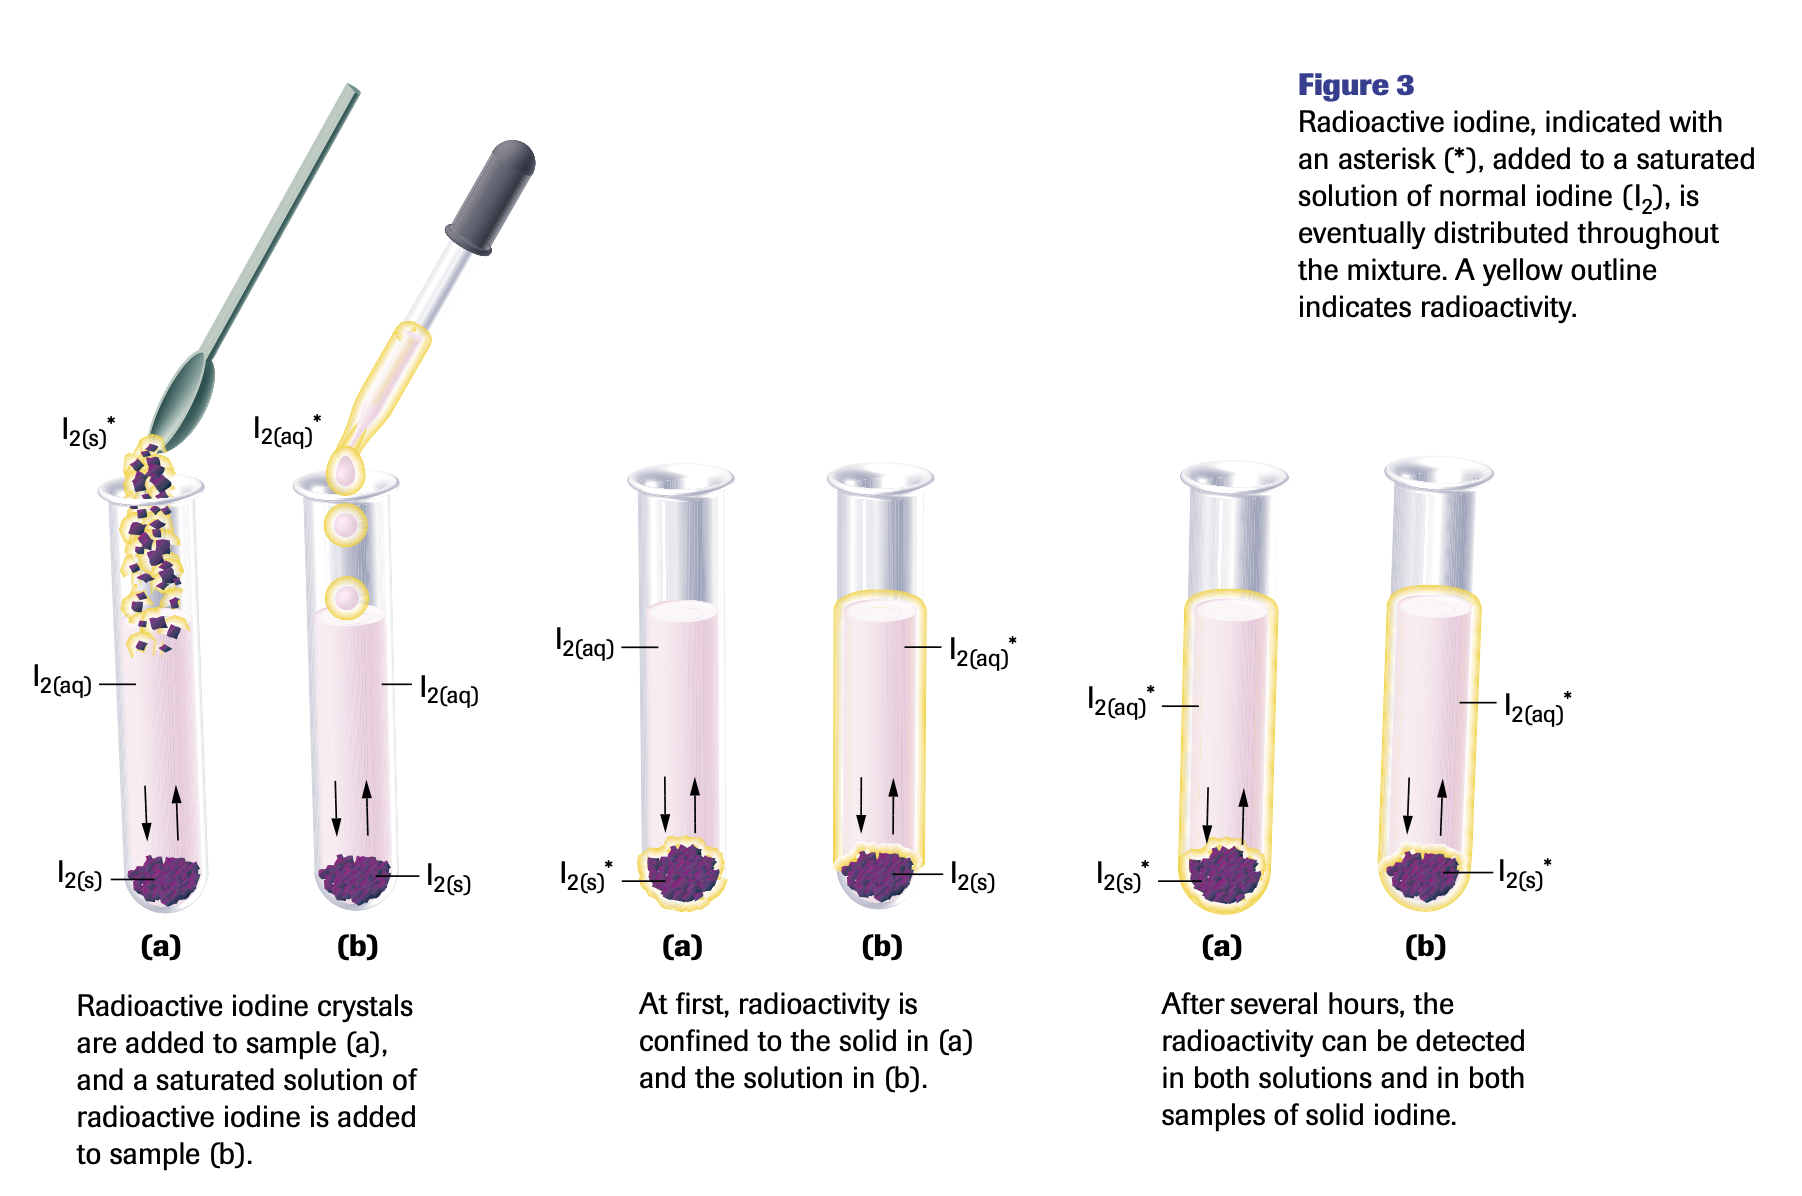
\includegraphics[width=0.8 \textwidth]{../figures/radioactive-iodine-solubility-equilibrium.png}
    \caption{(a) contains solid unsaturated radioactive idoine and (b) contains saturated radioactive
    iodine. Both are mixed in normal iodine solution. Initially, only the iodine solids in (a) and
    the solution in (b) are radioactive. However, over time, in both cases (a) and (b), both the
    solid and solution components are radioactive.}
    \label{fig:radioactive-iodine-solubility-equilibrium}
\end{figure}

\begin{important}
    At equilibrium, the forward rates and reverse reaction rates are equal. How we achieved
    equilibrium is not relevant. For instance, once equilibrium is achieved, it is impossible to
    tell if we started with separate solutions of $\ch{Ca^{2+}_{(aq)}}$ and $\ch{SO4^{2-}_{(aq)}}$,
    or with excess $\ch{CaSO4_{(aq)}}$ added to pure water. Initially, the difference is evident,
    but once the equilibrium is achieved, assuming that the equilibrium positions are identical, 
    there is no difference.
\end{important}

\subsection{Phase Equilibrium}
\begin{bulleted-list}
    \item An example of \textbf{liquid-gas equilibrium} is having a water bottle with the cap closed. A small
        percentage of liquid water molecules have enough kinetic energy to change into gaseous state.
        However, simultaneously, there are also gaseous water molecules that are colliding with the
        liquid water molecules, causing them to turn also into liquid water molecules. In this case,
        the rate at which both processes are occuring are identical, thus no change is observed
    \item If the lid was uncapped however, the system becomes an open system and the liquid water
        will eventually all become gaseous liquid water molecules
    \item \textbf{Note:} the tendency of any liquid to evaporate increases at higher temperatures,
        so the concentration and pressure of the vapour is greater if the equilibrium is established
        at a higher temperature
    \item An example of \textbf{solid-liquid equilibrium} is ice/water slush at 0$^{\circ}$C and
        101.325 kPa. As the temperature of the water drops, the rate of melting decreases while the
        rating of freezing increases simultaneously, until a temperature of 0$^{\circ}$C, where the
        rates become equal and the mixture will remain constant
\end{bulleted-list}

\subsection{Chemical Reaction Equilibrium}
\begin{bulleted-list}
    \item \textbf{Quantitative reaction:} a chemical reaction in which virtually all of the limiting
        reagent is consumed. Often occurs in an \textbf{open system}
    \item A synthesis/decomposition reaction are common types of reversible reactions
    \item \textbf{Reversible reaction:} a reaction that can achieve equilibrium in the forward
        or reverse direction. Occurs in a \textbf{closed system}
\end{bulleted-list}

\subsection{Percent Reaction at Chemical Equilibrium}
\textbf{Percent reaction:} the yield of product measured at equilibrium compared to the maximum 
possible yield of product.\\

All chemical reactions are considered reversible; the only thing to consider is the extent to which
they are reversible. Reactions fall loosely into three categories
\begin{bulleted-list}
    \item Reactions that favour reactants strongly; the percent reaction is less than
        1\%. In these reactions, mixing the reactants has no observable effect
    \item Reactions that favour products very strongly; where the percent reaction is greater than
        99\%. These reactions are observed to be quantitative reactions. These reactions are typically
        written with an arrow that has only one direction, to show that their reverse reaction is
        negligible
    \item Reactions that achieve noticeable equilibrium; the percent reaction lies somewhere
        between 1\% and 99\%. Only occurs in a closed system. If the percent reaction is less than
        50\%, reactants are favoured; if the percent reaction is more than 50\%, the products
        are favoured
    \item An ICE table, standing for initial, change, and equilibrium, is useful for calculating
        stoichoimetry involving dynamic equilibrium
\end{bulleted-list}
